% !TeX root = ../report.tex

\section{Feature based approach}

For the feature based approach, a feature extraction is done with regards to the term frequency - inverse document frequency. This has been the golden standard [CITE, speach and language processing page 278] for feature extraction, and ensures that the features extracted have the highest descriptive effect with regards to the tweets in which the feature occurs versus the tweets in which the feature does not. These extracted features are then used for the training of one of two different models, depending on the subtask at hand.\\
Both models builds on the random forest learning method since its properties supports both regression and multi-label classification. \\
The two models share the same general feature extraction, so they can be made directly comparable if the extraction parameters are kept comparatively the same.

\subsection{Custom features}
Besides the Tf-idf feature extraction method, we have implemented our own custom feature extraction function. In this function we have different flags, corresponding to different features that could be of interest in these particular tweets. \\
These different custom features involves e.g. whether or not a hashtag is present or if the spelling error of the whole tweet is above some threshold set by us. All of these custom features are boolean values in the sense that they are either present or not. \\
These features are then appended to the feature matrix returned by the Tf-idf extraction function, so that they are taken into consideration when training the different models. \\
Custom features can be based on linguistic and contextual intuition as well as a higher degree of linguistic analysis, as opposed to the deep learning features which will be trained with a more mathematically and statistical paradigm in mind.

\subsection{Model overview}
All the models share the same feature extraction method and the actual models were implemented using libraries which allowed a very high level approach. This acted as an introduction to the subtasks and which ones would be interesting to focus on and also as a baseline system which would work as a stepstone for the deep learning models used later in the process. In the final version of the code, two feature based models were used:\\
\begin{itemize}
 \item Random forest classifier
 \item Random forest regressor
\end{itemize}

\subsection{Results and data}
\begin{figure}[H]
    \centering
        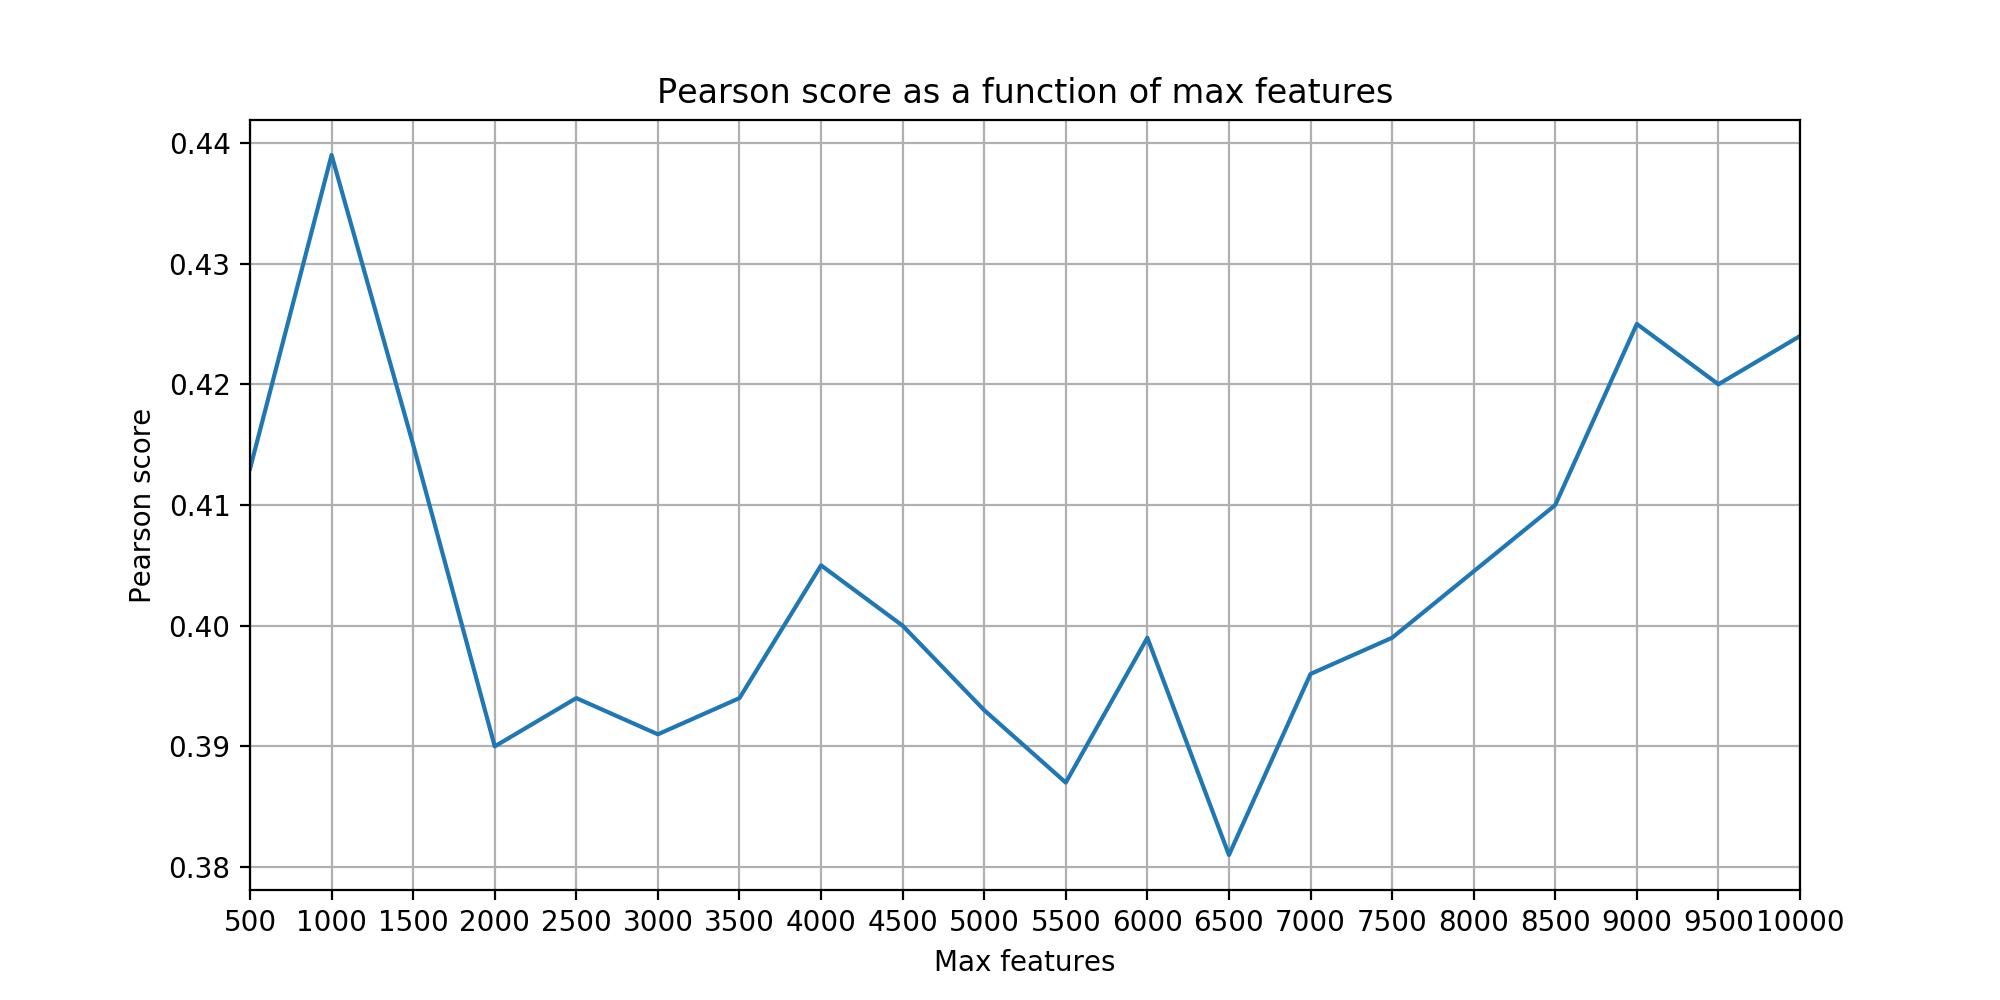
\includegraphics[width=\textwidth]{pictures/max_f_ngram15_hashtag.png}
        \caption{Pearson score as a function of max-features from 500-10000 with n-gram range 1-5 and hashtag custom feature}
        \label{fig:max_f_ngram15_hashtag}
\end{figure}